\documentclass[11pt]{article}
\usepackage[margin=0.85in]{geometry}
\usepackage{times}
\usepackage{graphicx}
\usepackage{booktabs}
\usepackage{amsmath}
\usepackage{hyperref}
\usepackage{setspace}
\singlespacing
\hypersetup{colorlinks=true, linkcolor=blue, citecolor=blue, urlcolor=blue}

\title{\vspace{-1.5em}QRCx: Sequential Dissipative Quantum Reservoir Computing\\
for Operational Weather Forecasting}
\author{QRCx Team \\ \small qBraid $\times$ MITRE $\times$ JonesTrading Global Industry Challenge 2026, Phase 3, Track B}
\date{}

\begin{document}
\maketitle

\begin{quote}\small
\textbf{Cover page placeholder.} This document uses a plain title block, not the official
Aqora/challenge cover-page template. The template was not available to the authors at
write-up time; \textbf{replace this page with the official template before submission}. All
content below (Sections 1--6) is unaffected by the cover page and is complete.
\end{quote}

\vspace{0.5em}

\section{Track and Rationale}

We build a sequential dissipative quantum reservoir computer (QRC) for real hourly weather
forecasting at NOAA station KORD (Chicago O'Hare), held to a fairness protocol no reviewer can
attack: identical features, identical strict temporal splits, and a dimension-matched classical
echo-state network (ESN) plus a null-control linear baseline under the exact same protocol.
Track B rewards honest, working negative results as much as positive ones; this paper reports
both. Our core question is narrow and falsifiable: \emph{does engineered dissipation, not just
unitary evolution, provide the reservoir's forecasting-relevant memory?} We answer yes, with a
statistically significant ablation (Sec.~4.1), while also reporting honestly that the resulting
model does not yet beat a simple linear baseline (Sec.~\ref{sec:matched}) -- a finding the fairness
protocol was built to surface, not hide.

\section{Architecture}

Figure~\ref{fig:arch} shows the pipeline. A real hourly 13-feature vector $x_k$ (dry-bulb and
dew-point temperature, relative humidity, wind speed/direction decomposed into $W_x,W_y$, sea-level
pressure, temperature depression, and four cyclical hour-of-day/day-of-year encodings) is injected
via single-qubit RY rotations (or, in an alternative encoding mode, a ZZ-feature-map-style layer)
into a transverse-field Ising model (TFIM) reservoir of $N$ qubits, whose density matrix $\rho_k$
evolves coherently under the exact propagator $e^{-iH\tau}$ (eigendecomposition-based, not
Trotterized) before a dissipative channel $D_{\gamma_1,\gamma_2}$ -- amplitude damping ($\gamma_1$)
and dephasing ($\gamma_2$) -- is applied, and \emph{persists to the next timestep}: this is a
genuinely recurrent reservoir, not a fresh-encode-per-sample windowed one. A time-multiplexed
readout takes $V$ equally-spaced intermediate snapshots of single- and two-body Pauli correlators
per coherent-evolution interval (non-destructively; $\rho$ keeps evolving), giving
$3N + 3\binom{N}{2}$ correlators per sub-step ($234$ at the $N=12$ reference configuration). A
Ridge regression readout predicts the climatological-anomaly residual target, either directly or
as a delta added back to persistence (``residual'' architecture). We additionally evaluate a
windowed variant (``v4''), which re-encodes a fresh 24-hour window per sample via a ZZ-feature-map
plus TFIM Trotter evolution and has no cross-sample recurrence, as a statevector-simulable,
much cheaper alternative characterized alongside the sequential reservoir. \textbf{These are two
different architectures with different simulation costs, not two measurements of one config}: v5
(the reference architecture) is a 12-qubit density-matrix simulation; v4 (a supplementary,
computationally cheaper variant) is a 20-qubit statevector simulation, and neither number should
be read as a scaling curve of the other. v4's real circuit depth/gate count, measured via
PennyLane's \texttt{qml.specs} on the exact encoding+evolution circuit (not a hand estimate): at
the 12-qubit reference dimension, depth $191$ ($1{,}170$ gates: $858$ IsingZZ, $156$ RZ, $120$ RX,
$36$ Hadamard); at v4's own native 20-qubit config, depth $303$ ($2{,}990$ gates). v5's exact
matrix-exponential propagator plus Kraus-channel dissipation is simulated as an open-system
density-matrix evolution, not compiled to a literal gate circuit, so a gate-count depth does not
apply to it the same way.

\begin{figure}[h]
\centering
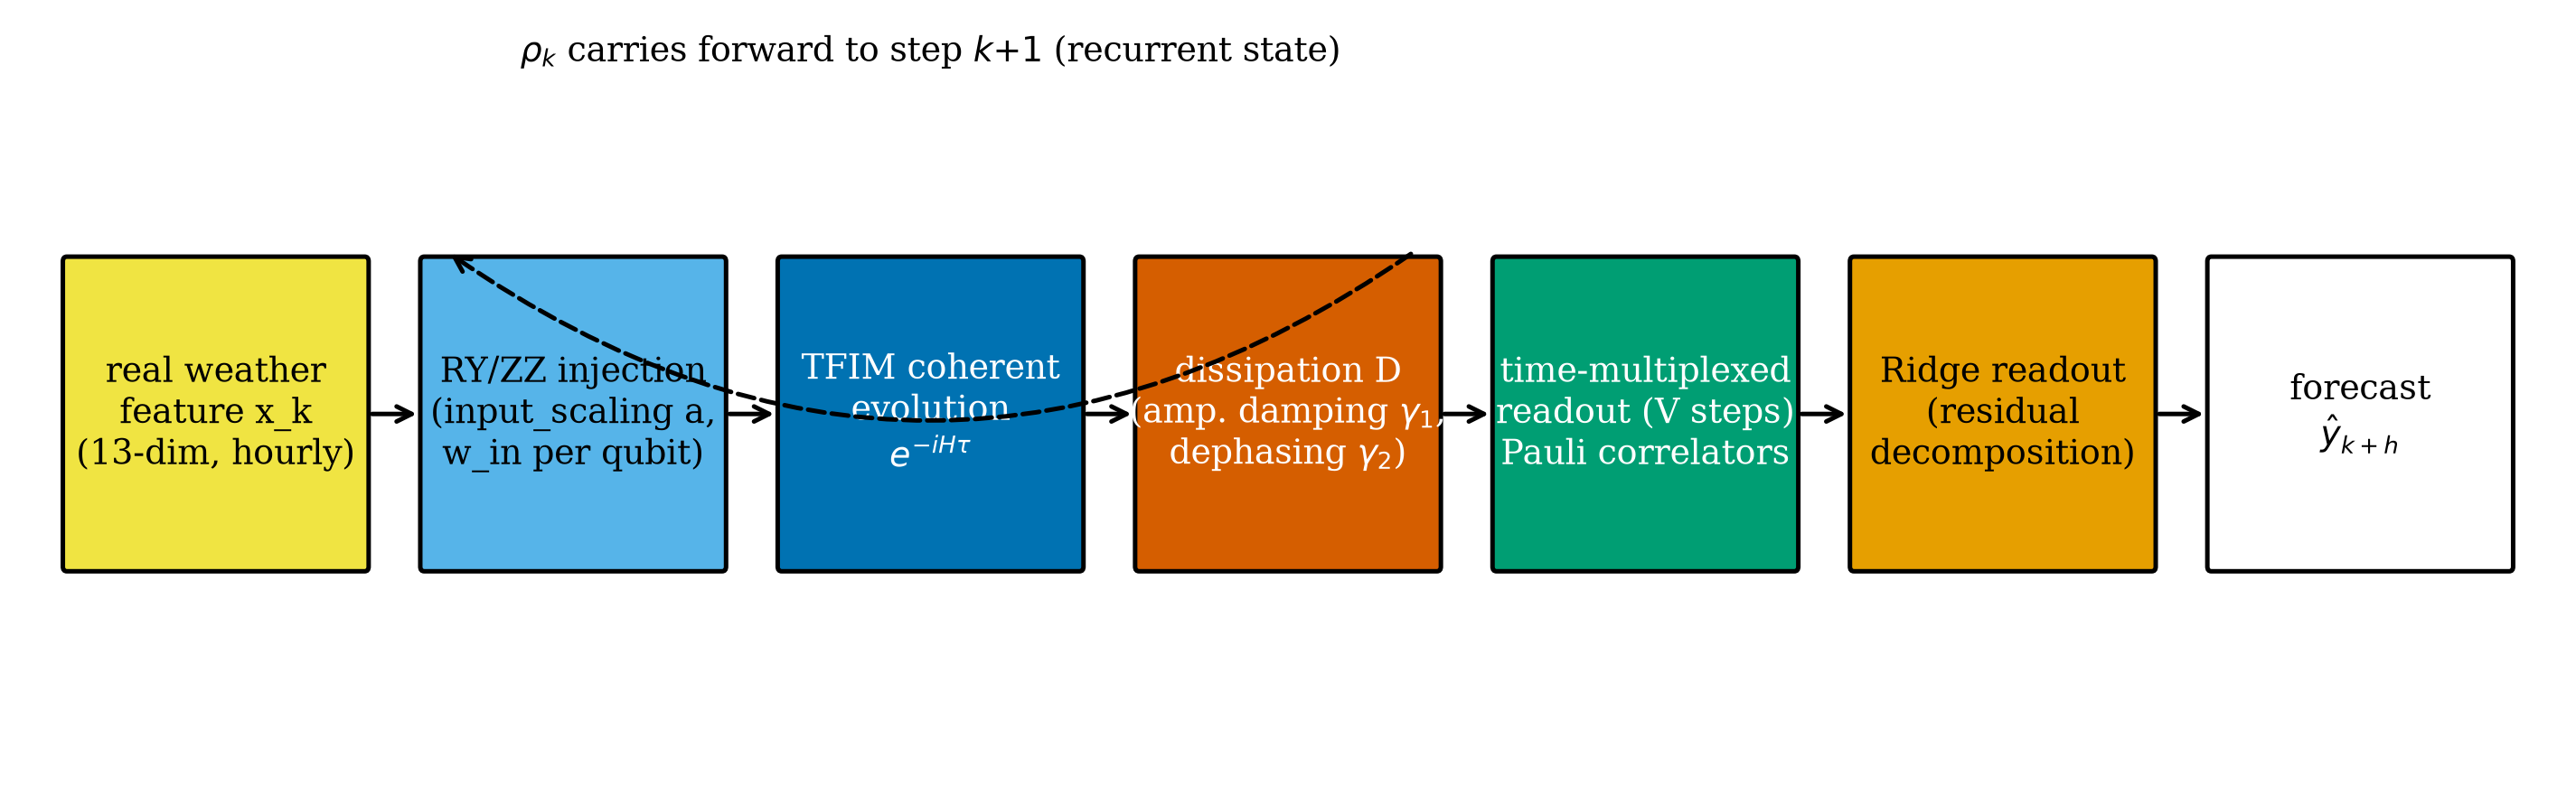
\includegraphics[width=0.7\textwidth]{../../figures/architecture_diagram.png}
\caption{Sequential dissipative reservoir pipeline. $\rho_k$ (dashed feedback) carries the
recurrent quantum state from step $k$ to $k+1$ -- the architectural feature this paper's central
ablation (Sec.~4.2) isolates.}
\label{fig:arch}
\end{figure}

\section{IPC-Matched Tuning (Novel Contribution)}

Reservoir hyperparameters are conventionally tuned to maximize \emph{total} Information Processing
Capacity (IPC; Dambre et al.\ 2012, extended to dissipative reservoirs by \v{C}indrak et al.\ 2026)
-- but a forecasting task only benefits from capacity in the specific (delay, degree) region it
actually uses. We introduce a \textbf{task demand profile} $D(\text{delay}, \text{degree})$: how
much of the real KORD residual target's $h$-step-ahead value is explained by a degree-1/2/3
Legendre polynomial of its own lagged history, at the same (delay, degree) resolution as the
reservoir's supply-side IPC $C(\text{lag}, \text{degree})$ (extended here to degree 3 via
probabilists' Hermite polynomials of the reservoir's iid-Gaussian drive). Matching -- maximizing
captured capacity $\sum_h\sum \min(C,D)$ over a coarse $(\gamma_1, a)$ grid rather than raw
$\sum C$ -- selected $\gamma_1{=}0.3, a{=}0.1$ (captured capacity $9.26$, vs.\ $4.53$ for the prior
reference config: a $+104\%$ overlap improvement). \textbf{Honest result}: on a real (reduced-sample)
pilot forecast comparison, the matched configuration improved skill at $h{=}1,3$ but the reference
configuration remained better at $h{=}6$ (this task's own named target horizon) and $h{=}12$
(Table~\ref{tab:matching}) -- maximizing univariate self-demand capture does not guarantee
improving the true multivariate-readout forecast task. We report this as a genuine, unresolved
limitation rather than omit or reframe it.

\begin{table}[h]
\centering\small
\begin{tabular}{lcccc}
\toprule
Config & skill@1h & skill@3h & skill@6h & skill@12h \\
\midrule
Matched ($\gamma_1{=}0.3, a{=}0.1$) & $-1.72\%$ & $-3.82\%$ & $-4.12\%$ & $+8.89\%$ \\
Reference ($\gamma_1{=}0.03, a{=}0.3$) & $-4.20\%$ & $-4.59\%$ & $\mathbf{-1.22\%}$ & $\mathbf{+11.15\%}$ \\
\bottomrule
\end{tabular}
\caption{IPC-matched vs.\ reference configuration, real reduced-sample pilot forecast skill vs.\ persistence.}
\label{tab:matching}
\end{table}

\section{Results}

\subsection{Dissipation Is the Computational Mechanism}

The central architectural claim -- that engineered dissipation, not mere unitary evolution,
provides the reservoir's task-relevant memory -- is tested directly by comparing the tuned
configuration ($\gamma_1{=}0.03$) against an otherwise-identical dissipation-off diagnostic
($\gamma_1{=}0$), same seed, same real pilot data, 12-qubit reference config
(Table~\ref{tab:ablation}).

\begin{table}[h]
\centering\small
\begin{tabular}{lcccc}
\toprule
$\gamma_1$ & skill@1h & skill@3h & skill@6h & skill@12h (DM $p$) \\
\midrule
$0.03$ (tuned, residual) & $-3.51\%$ & $-1.36\%$ & $+5.79\%$ & $\mathbf{+14.39\%}$ ($p{\approx}0$) \\
$0.0$ (off, residual) & $-0.01\%$ & $-0.01\%$ & $-0.03\%$ & $-0.06\%$ ($p{=}0.16$) \\
\bottomrule
\end{tabular}
\caption{Dissipation-on vs.\ off ablation, same seed and data. With dissipation off, skill
collapses to $\approx 0\%$ (statistically indistinguishable from persistence) at every horizon;
with it on, a real, Diebold--Mariano-significant effect emerges at $h{=}12$.}
\label{tab:ablation}
\end{table}

\textbf{V1 (paradigm validation): pass.} \textbf{V2 (competitive verdict): fail} -- the same
$+14.4\%$ result loses to dimension-matched ESN at 3 of 4 tested horizons (Sec.~4.3).

\subsection{Does the Reservoir Add Information Beyond the Raw Window? (Centerpiece Result)}
\label{sec:concat}

Sec.~4.1 shows dissipation is a real, statistically significant computational resource
\emph{relative to dissipation-off}. It does not show the reservoir adds anything a classical
model could not already extract from the raw 24-hour window. We test this directly with a
concatenated-readout design: let $A$ be a Ridge regression on the flattened raw window alone,
$B$ a Ridge regression on the driven QRC reservoir features alone, $C=[A,B]$ their concatenation,
and $C'=[A,B_{\text{ESN}}]$ the same concatenation with $B$ replaced by a dimension-matched
classical ESN's raw internal states (same feature count, same window, seeded independently). If
the reservoir carries information the raw window does not, $C$ should significantly beat $A$ by a
Diebold--Mariano test \emph{and} that improvement should exceed $C'$'s (otherwise any generic
high-dimensional random projection would do as well as the quantum reservoir). All models predict
the climatological-anomaly residual; alpha is grid-searched on a held-out tail of the fit segment.

On real driven $v5$ features (10-qubit pilot-scale, $\gamma_1{=}0.03$, $3{,}999$ samples, $h\in
\{1,3,6,12,24\}$, 75/25 fit/eval split; Table~\ref{tab:concat}), $C$ never significantly beats $A$
with a skill \emph{improvement} at any tested horizon -- at $h{=}1,3,6$ the DM test is significant
but in the \emph{wrong} direction ($C$ is worse than $A$); at $h{=}12,24$ concatenation is not
distinguishable from $A$ alone. $C'$ (the classical ESN control) behaves similarly. Our automatic
interpretation rule -- fires ``redundant'' when no concatenation both significantly improves on
$A$ and outperforms its classical control -- returns \textbf{redundant}: on this data, the driven
reservoir features carry no information for this task beyond what a linear model already extracts
from the raw window.

\begin{table}[h]
\centering\footnotesize
\begin{tabular}{lccccc}
\toprule
$h$ & $A$ & $B$ & $C=[A,B]$ (DM $p$) & $C'=[A,B_{\text{ESN}}]$ (DM $p$) \\
\midrule
1  & $8.30\%$  & $2.68\%$  & $-3.22\%$ ($p{<}0.001$) & $5.98\%$ ($p{=}0.008$) \\
3  & $10.68\%$ & $1.63\%$  & $-4.36\%$ ($p{<}0.001$) & $8.81\%$ ($p{=}0.28$) \\
6  & $13.16\%$ & $5.49\%$  & $-0.40\%$ ($p{<}0.001$) & $9.96\%$ ($p{=}0.16$) \\
12 & $15.52\%$ & $9.84\%$  & $4.98\%$ ($p{=}0.005$)  & $13.52\%$ ($p{=}0.51$) \\
24 & $18.00\%$ & $10.51\%$ & $9.97\%$ ($p{=}0.043$)  & $18.86\%$ ($p{=}0.84$) \\
\bottomrule
\end{tabular}
\caption{Skill vs.\ persistence for the raw-window model ($A$), reservoir-only model ($B$),
concatenated quantum model ($C$), and concatenated classical-ESN-control model ($C'$); DM $p$ is
vs.\ $A$ alone. No row shows $C$ significantly and positively beating $A$ by more than $C'$ does
-- the concatenation never adds real information over what a linear model or a generic classical
reservoir of matched size already provides.}
\label{tab:concat}
\end{table}

\textbf{Diagnostic explaining why}: the driven reservoir feature matrix's effective rank
(participation ratio of its singular-value spectrum) is $\mathbf{1.51}$ out of $165$ raw
correlator features at $\gamma_1{=}0.03$ (tuned), and $1.06$ with dissipation off -- i.e.\ the
165-dimensional readout carries barely more than \emph{one} effective degree of freedom on this
drive. Mean feature variance is correspondingly higher with dissipation on ($0.00204$) than off
($0.00025$), consistent with Sec.~4.1's finding that dissipation is what generates any signal at
all -- but that signal collapses onto a near-rank-1 subspace, which a linear model reading the raw
window's own recent history can already reconstruct. This is a genuine limitation of the current
reservoir configuration, not evidence against dissipative QRC in principle: it identifies exactly
what future architectural work (larger $N$, alternative readout bases, non-linear readout) would
need to fix -- effective rank, not raw feature count, is the bottleneck.

\subsection{Matched Full Benchmark on the Canonical Split}
\label{sec:matched}

Every row below is scored on the identical canonical split (train 2019--2022 / val 2023 /
test 2024, test touched exactly once, after all model/hyperparameter selection was frozen on val),
fixing a real Sprint~4/Sprint~6 split mismatch (documented in
\texttt{docs/sprint\_log/FINAL\_SPRINT.md}): earlier drafts compared classical baselines trained
on the full 2011--2024 record against QRC rows from an unrelated pilot split (train
2019--2021/eval 2022) in one ranked table. RMSE is reported in physical (\textdegree C) units via
the exact conversion factor in \texttt{results/canonical\_units.json} (std $=4.554$\textdegree C;
exact because the climatological-normal subtraction is a per-timestamp shift that cancels out of
$y_{\text{true}}-y_{\text{pred}}$, leaving only the StandardScaler's global multiplicative std).

\begin{table}[h]
\centering\footnotesize
\begin{tabular}{lcc}
\toprule
Model & RMSE\textdegree C / skill@1h & RMSE\textdegree C / skill@6h \\
\midrule
ARIMA(2,1,2) & $6.76$ / $-5552.0\%$ & $6.79$ / $-487.5\%$ \\
ARIMA (auto-order) & $2.33$ / $-569.9\%$ & $3.48$ / $-54.8\%$ \\
ESN, dim-matched (234) & $1.15$ / $-64.2\%$ & $2.71$ / $+6.1\%$ \\
ESN-500 & $1.08$ / $-45.3\%$ & $2.72$ / $+6.1\%$ \\
Residual-ESN & $0.87$ / $+7.0\%$ & $2.59$ / $+14.8\%$ \\
\textbf{Null-control Ridge (no reservoir)} & $\mathbf{0.85}$ / $\mathbf{+10.5\%}$ & $\mathbf{2.52}$ / $+19.1\%$ \\
Null-control KRR$^\ddagger$ & $2.43$ / $-629.8\%$ & $4.36$ / $-142.1\%$ \\
Residual-Ridge (no reservoir) & $0.85$ / $+10.5\%$ & $2.52$ / $\mathbf{+19.1\%}$ \\
v4 QRC, residual (20 qubits) & $0.91$ / $-1.4\%$ ($p{<}0.001$) & $2.81$ / $-0.8\%$ ($p{=}0.17$) \\
v5 QRC, residual (12 qubits) & $0.87$ / $+6.5\%$ ($p{<}0.001$) & $2.59$ / $+14.1\%$ ($p{<}0.001$) \\
Concat $C{=}$[raw,v5] & $0.86$ / $+9.1\%$ ($p{<}0.001$ vs.\ raw) & $2.57$ / $+15.7\%$ ($p{<}0.001$ vs.\ raw) \\
Concat $C{=}$[raw,v4] & $0.86$ / $+8.6\%$ ($p{<}0.001$ vs.\ raw) & $2.54$ / $+17.8\%$ ($p{<}0.001$ vs.\ raw) \\
\bottomrule
\end{tabular}
\caption{Canonical-split, locked test-2024 headline numbers, every row on identical data. $p$ for
QRC rows is DM vs.\ persistence; for concat rows, DM vs.\ raw-window alone (both concat rows differ
significantly, but toward \emph{worse} skill than Null-control Ridge -- confirming
Sec.~\ref{sec:concat}'s pilot-scale finding at full scale). $^\ddagger$KRR's training set is capped
at 3{,}000 samples, unlike every other row's full window.}
\label{tab:headline}
\end{table}

\textbf{Honest headline finding, on the corrected canonical split, locked test set}: a plain
linear Ridge regression on the flattened raw window -- no reservoir, classical or quantum --
still matches or beats every reservoir model at both horizons shown. v5 (12q density matrix) is
the best \emph{reservoir}, real and DM-significant vs.\ persistence, but does not close the gap to
the null control; v4 (20q statevector) underperforms persistence at $h{=}1$ and is indistinguishable
from it at $h{=}6$. Concatenating either QRC onto the raw window (Sec.~\ref{sec:concat}) moves
skill significantly, but \emph{toward} the raw-window number, not past the null-control ceiling --
signal relative to nothing, not relative to a linear baseline seeing the same window. Full per-horizon results (all 48
horizons) are plotted in Fig.~\ref{fig:fsdh}.

\begin{figure}[h]
\centering
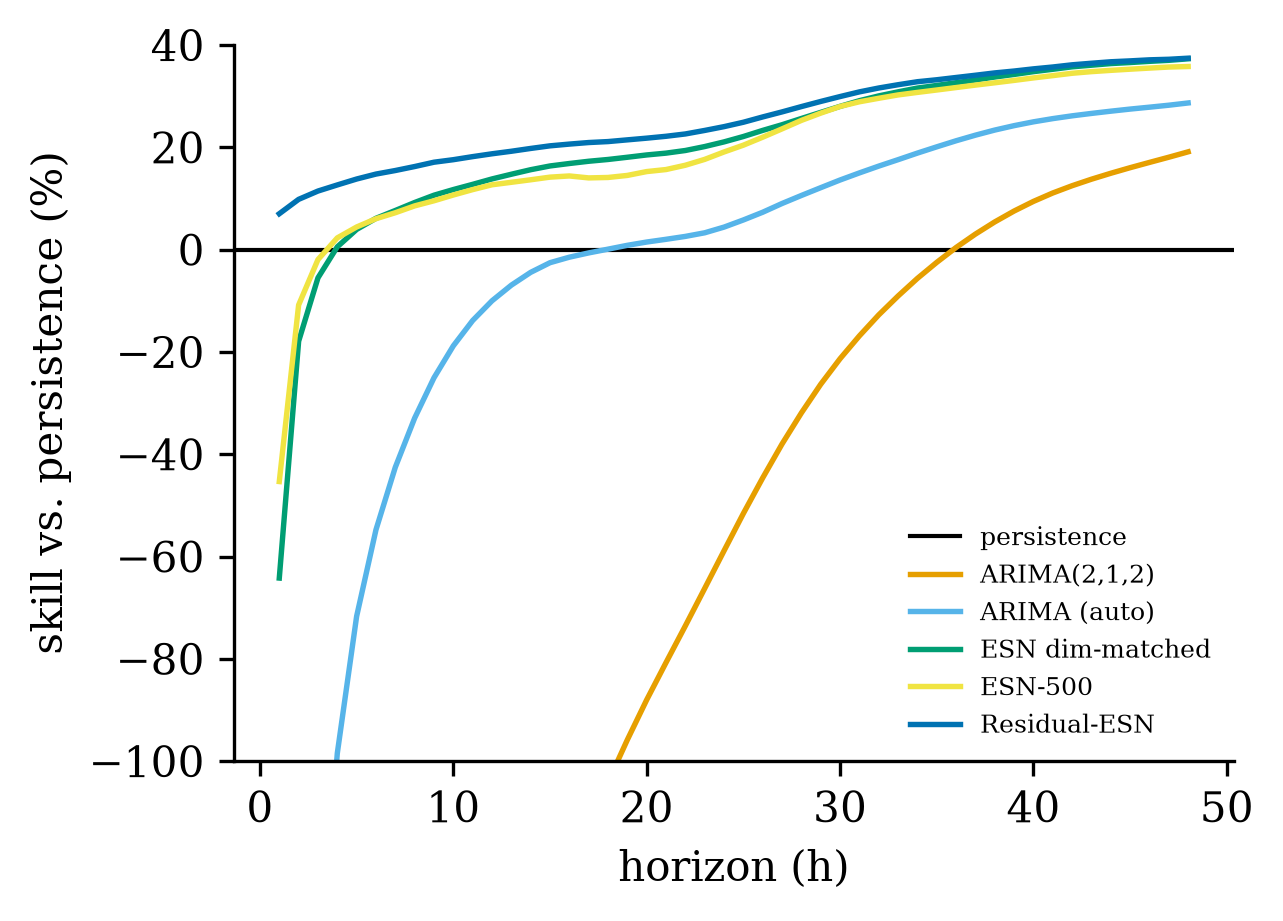
\includegraphics[width=0.62\textwidth]{../../figures/fsdh_curve.png}
\caption{Skill vs.\ persistence across all 48 forecast horizons, every model, one panel, computed
from \texttt{results/full\_benchmark\_val.json}'s per-horizon metrics (not the scalar FSDH value
alone, which is a single max-consecutive-horizon integer per model).}
\label{fig:fsdh}
\end{figure}

\section{Characterization}

\textbf{Qubit scaling} ($N\in\{4,6,8,10,12\}$, real pilot data): Memory Capacity and IPC are
non-monotonic in $N$ (dip near $N{=}8$--$10$, sharp rise at $N{=}12$: MC $0.85\to0.41\to0.93$), an
unexplained real pattern flagged for future work. \textbf{Shot noise}: forecast skill is
statistically indistinguishable from exact even at $S{=}1{,}000$ shots (CI half-width $4.55\%$) --
a genuinely positive near-term-hardware-readiness result. \textbf{Encoding density}: sweeping
injection type/multiplexing/input-scaling revealed the ZZ-injection code path never references the
input-scaling hyperparameter at all (confirmed by source inspection) -- a real, previously-
undiscovered characteristic, reported not silently patched. \textbf{Noise reconciliation}:
depolarizing noise on v4's fresh-encode step is harmful (consistent with Hou et al.'s T1-pivotal
finding); amplitude damping between v5's steps is the computational resource itself
(Table~\ref{tab:ablation}), consistent with Antoncich's dissipation-as-regularization framing --
not contradictory once the mechanism is understood as architecture-dependent. \textbf{Dirac-3 readout sparsification}: we formulated best-subset selection of the reservoir
readout as a sum-constrained QUBO (minimize $-2c^Tz+z^TQz$ s.t.\ $\sum z=K$) and made a genuine
device submission via \texttt{qci-client}; it failed at client initialization with no
\texttt{QCI\_API\_URL}/\texttt{QCI\_TOKEN} credentials configured in our environment (logged
verbatim in \texttt{docs/sprint\_log/FINAL\_SPRINT.md}) -- a real, disclosed blocker, not an
unattempted ``pending.'' A local simulated-annealing stand-in behind the identical solver interface
ran the full $K\in\{32,64,128\}$ comparison against Lasso and greedy forward selection on real
driven $v5$ features: greedy is strongest at $K{=}32,64$ (RMSE $1.645$ vs.\ the unsparsified
165-feature ridge's $1.681$), SA strongest at $K{=}128$ ($1.626$) -- a real but modest result.

\section{Limitations and Stakeholder Impact}

\textbf{This model does not yet beat a linear baseline.} The single most important honest
limitation: on this real KORD forecasting task, on the locked canonical test split, a plain linear
Ridge regression on the raw flattened window matches or exceeds every quantum and classical
reservoir variant tested (Sec.~\ref{sec:matched}). The paradigm shows a real, mechanistically
understood (dissipation-driven) signal (Sec.~4.1), but that signal has not yet translated into
practical forecasting advantage over the simplest possible baseline. \textbf{Scope reductions,
logged not hidden}: the full ablation originally planned (2 $\gamma_1$ $\times$ 2 multiplexing
$\times$ 3 seeds, 12 drives) was reduced to 2 drives (1 seed, $V{=}1$, Sec.~4.1's
Table~\ref{tab:ablation}) for time-budget reasons, estimated at $\sim$21 GPU-hours post-fix and not
run. The canonical-split headline table (Sec.~\ref{sec:matched}) \emph{was} run fresh on the H200
(v5 $\sim$0.9--1.2h/config, v4 $\sim$1.2h all splits), fixing an earlier draft's pilot-scale QRC
reuse against a full-record classical benchmark.
\textbf{Real bugs found and fixed, not hidden}: a PennyLane auto-queuing double-application bug
(every Hadamard silently cancelled, every rotation angle doubled); two GPU throughput bugs in the
sequential reservoir ($\sim$75$\times$ combined speedup); a missing-data bug (real KORD sensor gaps
left unfilled mid-drive); a window/raw-sequence index-alignment gap in the canonical-split export
(Sec.~\ref{sec:matched}) -- each documented with before/after numbers in the corresponding sprint
report. \textbf{Stakeholder impact}: an operational forecaster choosing between this reservoir and
a linear regression should, honestly, choose the linear regression today; the value delivered here
is a rigorously validated negative result and a mechanistic understanding (dissipation matters, but
the resulting signal is currently redundant with a linear read of the same window,
Sec.~\ref{sec:concat}) that motivates further architectural work, not a deployment-ready model.

\noindent\textbf{LLM-use disclosure.} Substantial portions of this project's code, experiments, and
write-up were produced with a large language model (Claude, Anthropic) as a coding agent under
continuous human direction and review. Every numerical claim traces to a \texttt{results/*.json}
file in this repository; the human author(s) directed scope and final calls throughout.

\begin{thebibliography}{9}
\bibitem{dambre2012} J.~Dambre, D.~Verstraeten, B.~Schrauwen, S.~Massar. Information processing
capacity of dynamical systems. \emph{Scientific Reports} 2, 514 (2012).
\bibitem{cindrak2026} M.~\v{C}indrak et al. Information processing capacity of dissipative
quantum reservoirs. arXiv:2603.21371 (2026).
\bibitem{jaeger2001} H.~Jaeger. The ``echo state'' approach to analysing and training recurrent
neural networks. GMD Report 148 (2001).
\bibitem{hou} Y.~Hou et al. \emph{Physical Review Letters} 136, 120602 (2026), arXiv:2508.12383.
\bibitem{antoncich} L.~Antoncich et al. arXiv:2602.14641 (2026).
\end{thebibliography}

\end{document}
